% !TeX root = ../main.tex

\chapter{Teoria da informação em análise de formas}

Neste capítulo apresentamos como  grandezas e medidas da teoria da informação podem ser utilizadas na descrição e na avaliação de similaridade de formas.

Iniciamos o capítulo apresentando a entropia de Shannon, a entropia diferencial e suas propriedades. 

Em seguida descrevemos a metodologia utilizada para obtenção de descritores de forma a partir dessas entropias.



\section{Entropia como descritor multiescala}

No capítulo \ref{chap:contour} mostramos como se obtém a curvatura multiescala como uma assinatura do contorno de uma forma. No mesmo capítulo apresentamos um descritor multiescala construído a partir da versão discreta dessa assinatura, mais especificamente a energia de dobramento multiescala. 

Aqui propomos dois novos descritores multiescala construídos a partir dessa mesma assinatura, mas explorando os conceitos de entropia discreta de Shannon e de entropia diferencial.

Para se obter tais descritores é necessário estimar as funções densidade de probabilidade do sinal da curvatura em diferentes escalas. No caso da entropia de Shannon, que tem em sua definição uma função densidade de probabilidade de massa, a maneira mais direta de se realizar tais estimativas é através de histogramas. Já no caso da entropia diferencial, empregamos para realizar tais estimativas o método da janela de Parzen.

\subsection{Entropia discreta da curvatura multiescala}

Sendo  $K[t,\sigma]$ a função curvatura multiescala do contorno de uma forma, discretizada em $M$ pontos e $U$ escalas, temos $\sigma = \{\sigma_1\text{, }\sigma_2\text{, }\ldots\text{, }\sigma_U\}$ como sendo os fatores de escala e $t = \{1\text{, }2\text{, }\ldots\text{, }M\}$ os índices dos possíveis valores da curvatura ao longo do perímetro do contorno. Fixada uma escala $\sigma'$ obtemos o histograma dessa função subdividindo o intervalo dos valores que a função curvatura multiescala pode assumir em $N$ faixas distintas de mesmo tamanho $\Delta x$ e contando o número de ocorrências dos valores dessa função dentro de cada uma dessas faixas  \cite{Webb:2002}. Desta forma, o valor de $\Delta x$ será   

\begin{equation}
\Delta x = \frac{\max\limits_{\forall t}{K[t,\sigma']}-\min\limits_{\forall t}{K[t,\sigma']}}{N}\text{,}
\end{equation}

 sendo o histograma

\begin{equation}\label{eq:histograma}
P\big(K[t,\sigma']\big) = \Big\{P_j|\:j = 1\text{, }2\text{, }\ldots\text{, }N\Big\}\text{, }
\end{equation}

%\begin{equation}
%P_\sigma[j] = \frac{n_j}{\sum\limits_{i=1}^Nn_i}\text{,}
%\end{equation}

 com $P_j=\frac{n_j}{\sum\limits_{i=1}^Nn_i}$ e $n_j = \#\{x \in \Re|\:\min\limits_{\forall t}{\big(K[t,\sigma']\big)}- j\Delta x \leq x \leq \min\limits_{\forall t}{\big(K[t,\sigma']\big)}+j\Delta x\}$. O operador $\#A$ denota a cardinalidade do conjunto A. 
 
 A entropia discreta da curvatura multiescala é obtida aplicando-se a equação \ref{eq:Shannon} ao histograma da função curvatura, obtido através da equação \ref{eq:histograma}, para os diferentes fatores de escala. Temos assim o descritor entropia discreta da curvatura multiescala como sendo
 
\begin{equation}
EDM = \big(H_{\sigma_1}\text{, } H_{\sigma_2}\text{, }\ldots\text{, }H_{\sigma_U}\big)
\end{equation}

aonde $H_{\sigma_u} = H(P_{\sigma_u})$ e $P_{\sigma_u} = P\big(K[t,\sigma_u]\big)$.
 
\subsection{Entropia diferencial da curvatura multiescala}

O cálculo da entropia diferencial da curvatura multiescala, através da equação \ref{eq:difent}, requer que se estime as funções densidade de probabilidade do sinal da curvatura em diferentes escalas.  A técnica não paramétrica da janela de Parzen pode ser utilizada para realizar tais estimativas. 
 
 Para uma dada escala $\sigma'$, temos a curvatura amostrada em $M$ valores como sendo $K[t,\sigma'] = \{K[1,\sigma']\text{, }K[2,\sigma']\text{, }\ldots\text{, }K[M,\sigma']\}$. A função densidade de probabilidade dessa função, estimada pela janela de Parzen, é dada por \cite{Webb:2002}:  
 
\begin{equation}\label{eq:parzen}
p_{\sigma'}(k) = \frac{1}{bM}\sum\limits_{i=1}^M\Psi(\frac{k - K[i,\sigma']}{b})\text{,}
\end{equation}

sendo $\Psi(z) = \frac{1}{\sqrt{2\pi}}\exp{-\frac{z^2}{2}}$ a função de janela e $b$ a sua largura de banda.

No processo de estimação através dessa técnica a escolha do parâmetro largura de banda é crítica, pois esse altera o grau de suavização da curva de densidade obtida. Valores elevados desse parâmetro tendem a suavizar em demasia a curva de densidade estimada acarretando em perda de detalhes importantes. Por outro lado, valores pequenos resultam em densidades estimadas com mais detalhes, porém mais ruidosa. Assim, é importante estabelecer um critério para escolha do parâmetro de largura de banda para que se tenha uma boa estimativa da função densidade de probabilidade. Adotamos neste trabalho o método proposto por Silverman \cite{silverman:1986}. Esse método, que determina uma escolha ótima de largura de banda, assume que a distribuição de probabilidade dos dados é normal e que a janela utilizada é gaussiana.

A largura de banda pelo método de Silverman é dada por \cite{silverman:1986}

\begin{equation}
b = \big(\frac{4\hat{\sigma}^5}{3n}\big)^\frac{1}{5}\text{,}
\end{equation}

sendo $\hat{\sigma}$ o desvio padrão e $n$ o número das amostras utilizadas no processo de estimação. 

Temos o cálculo da entropia diferencial da curvatura multiescala na escala $\sigma'$ aplicando o resultado obtido da equação \ref{eq:parzen} na equação \ref{eq:difent}, ou seja:

\begin{equation}\label{eq:desc_entropia}
h\big(K[t,\sigma']\big) = -\int_{-K_{min}}^{K_{max}}p_{\sigma'}(k)\log{p_{\sigma'}(k)}dk\text{, }
\end{equation}

sendo a integral calculada através do método numérico de integração de Simpson e os limites de integração $K_{min}$ e $K_{max}$ os valores máximos e mínimos da curvatura multiescala na escala $\sigma'$.

O descritor obtido a partir da equação \ref{eq:desc_entropia} apresenta propriedades de invariância a translação e a rotação. Isso porque a translação da forma não afeta o sinal da curvatura. Embora a rotação desloque em fase o sinal da curvatura, como ilustra a figura \ref{fig:curv_scale_rot}a, esse deslocamento não interfere na função densidade de probabilidade estimada, e portanto não interfere no cálculo do descritor.

Porém, o descritor não apresenta invariância a mudança de escala da forma. Isso porque tal mudança reflete em escala no sinal de curvatura (figura \ref{fig:curv_scale_rot}b), o que interfere na função densidade de probabilidade estimada, e portanto no cálculo do descritor.

Consegue-se a invariância do descritor à mudança de escala utilizando o perímetro da forma ($L_{\sigma'}$) como fator de normalização. Desta forma, aplicando a  propriedade da equação \ref{eq:escala_entropia}, temos a versão do descritor invariante a mudança de escala:

\begin{equation}\label{eq:entropia_inv}
\hat{h}\big(K(t,\sigma')\big) = -\int_{-K_{min}}^{K_{max}} p_{\sigma'}(k)\log{p_{\sigma'}(k)}dk+\log{L_{\sigma'}}\text{.}
\end{equation}

\begin{figure}[]
\caption{\label{fig:curv_scale_rot}Efeitos da rotação e da mudança de escala das formas sobre a curvatura.}
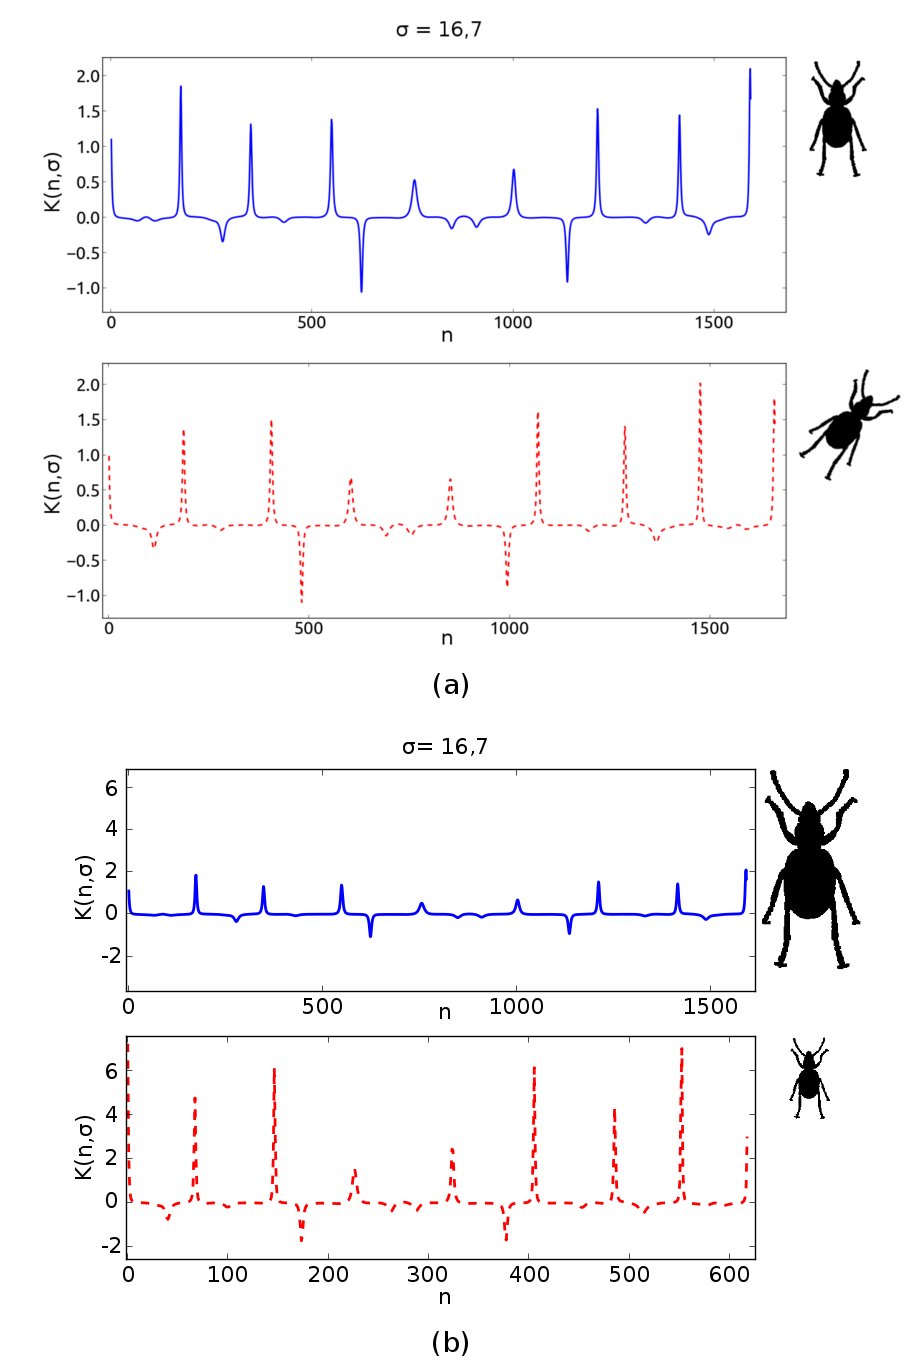
\includegraphics[width=\textwidth]{curvatura_scale_rot.png}
\legend{Fonte: próprio autor.}
\end{figure}

As figuras \ref{fig:entropia_inv}a e \ref{fig:entropia_inv}b ilustram o descritor entropia diferencial da curvatura multiescala, calculado para duas formas idênticas, em diferentes escalas. Na figura \ref{fig:entropia_inv}a o cálculo foi realizado através da equação \ref{eq:entropia_inv} e o descritor mostrou invariância à mudança de escala da forma. Já na figura \ref{fig:entropia_inv}b o cálculo foi realizado a partir da equação \ref{eq:desc_entropia} e o descritor não apresentou invariância à escala da forma.

A figura \ref{fig:entropia_inv}c ilustra a invariância do descritor à rotação da forma. Nesse caso, o cálculo foi realizado a partir da equação \ref{eq:entropia_inv}.

\begin{figure}[]
\caption{\label{fig:entropia_inv}Efeitos da rotação e da mudança de escala das formas sobre o descritor entropia diferencial da curvatura multiescala.}
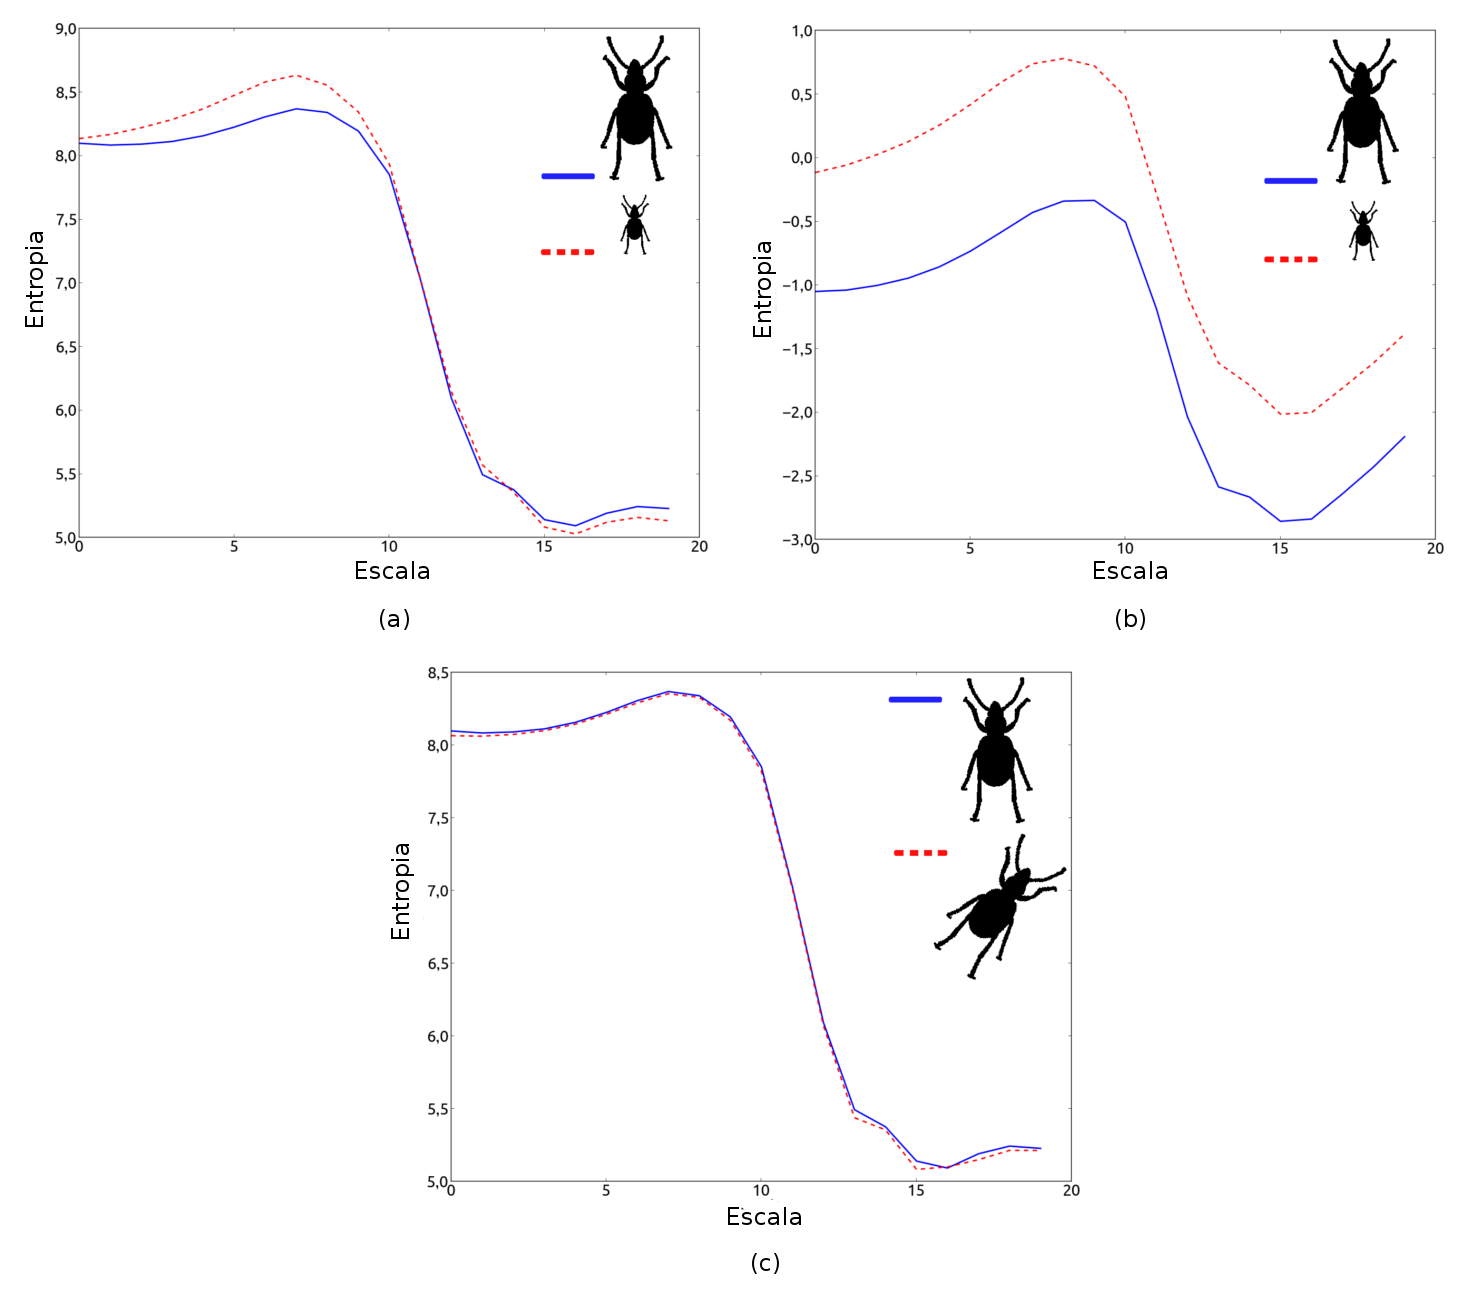
\includegraphics[width=\textwidth]{inv_entropia.png}
\legend{Fonte: próprio autor.}
\end{figure}

